%Correct the file name.
%X: book number
%Y: part number
%ZZZ: page number in three digits. So page 3 would be 003.

\documentclass[11pt]{amsbook}

\usepackage{../HBSuerDemir}	% ------------------------


\begin{document}
\setcounter{page}{65}

An element $e$ of a set $G$, on whichthere is a binary operation $\circ$, is called
a \textit{right identity element} or simply a \textit{right identity} if $a \circ e = a$ for all $a$ in

% ++++++++++++++++++++++++++++++++++++++
\hPage{feyzioglu/65}
% ++++++++++++++++++++++++++++++++++++++

$G$. The third group axiom (iii) ensures that group $G$ has a right identity
element. We will show presently that group has precisely one identity
element, but we have not proved it yet and we must be careful not to
use the uniqueness of the right identity before we prove it. All we know
at this stage is that a group has at least one right identity for which (iv)
holds. As it is, there may be many right identities. In addition, there
may be some right identities for which (iv) is true and also some for
which (iv) is false. For the time being, these possibilities are not
excluded. 

They will be excluded in Lemma 7.3, where we will prove further that
our unique right identity is also a left identity. A \textit{left identity element} or
a \textit{left identity} of $G$, where $G$ is a nonempty set with a binary operation $\circ$
on it, is by definition an element $f$ of $G$ such that $f \circ a = a$ for all $a \in G$.
The group axioms say nothing about left identities. If $(G, \circ)$ is a group,
we do not yet know if there is a left identity in $G$ at all, nor do we know
any relation between right and left identities. For the time being, there
may be no or one or many left identities in $G$. If there is only one left
identity, it may or may not be right identity. If there are many left
identities, some or one or none of them may be right identities. 

We mention all these possibilities so that the reader does not read in the
axioms more than what they really say. The group axioms say nothing
about left identities or about the uniqueness of the right identity. 

The group axioms do say something about right inverses. If $G$ is a
nonempty set with a binary operation $\circ$ on it, and if $e$ is a right identity
in $G$, and $a \in G$, an element $x \in G$ is called a \textit{right inverse} of $a$. (with
respect to $e$) when $a \circ x = e$. The group axioms state that, in case $(G, \circ)$ is
a group, there is a right identity $e$ in $G$ with respect to which each
element of $G$ has at least one right inverse. Until we prove Lemma 7.3,
there may be many right identities with this property. Also, some of the
right identity elements may and some of the right identity elements
may not have this property. Furthermore, some (or all) of the elements
may have more than one right inverses with respect to some (or all) of
the right identities. The group axioms make no uniqueness assertion
about the right inverses. 

Before we lose ourselves in chaos, we had better prove our lemma. 



% =======================================================
\end{document}  

%==== templates ====

%==== environments ====

%\begin{figure}[htb]
%	\centering
%	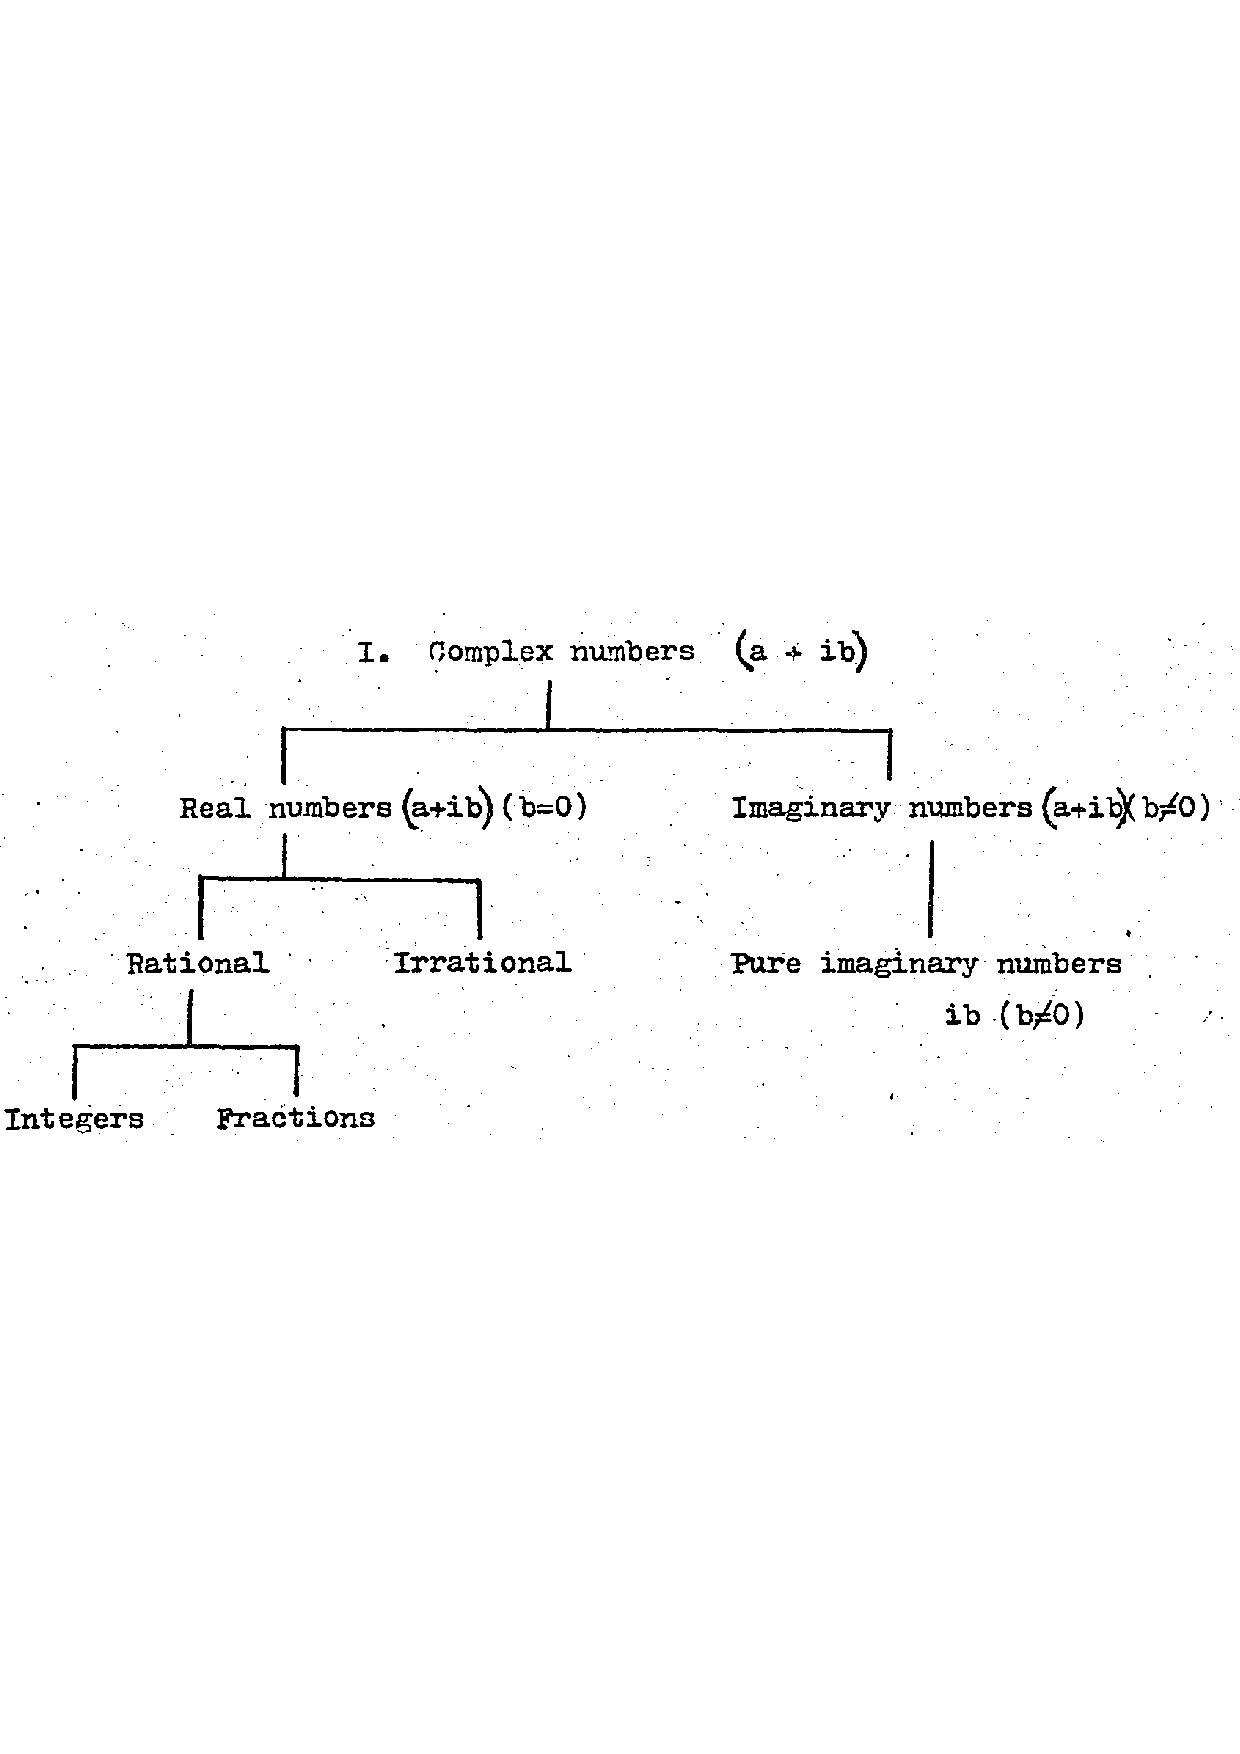
\includegraphics[width=0.9\textwidth]{images/SD-1-1p15A}
%	\caption{Classification of complex numbers}
%	\label{fig:classificationOfComplexNumbersA}
%\end{figure}

%\begin{center}
%\begin{tabular}{cc}
%\end{tabular}
%\end{center}

%\begin{exmp}
%\begin{hSolution}
%\end{hSolution}
%\end{exmp}

%\begin{hEnumerateAlpha}
%\end{hEnumerateAlpha}

%\begin{hEnumerateRoman}
%\end{hEnumerateRoman}

%$
%\begin{bmatrix}
%\end{bmatrix}
%$

%\frac{aaaa}{bbb}
%\frac{a_{n}}{b_{n}}
%\left( aaaa \right)
%\Longrightarrow

%\begin{multicols}{2}
%	bb
%\columnbreak
%	aa
%\end{multicols}
